\documentclass[conference]{IEEEtran}
\usepackage{graphicx}

\title{WitzWizard}
\author{krish, sanjayan, krith}

\begin{document}

\maketitle

\begin{abstract}
The proposed AI-assisted research writing system integrates academic text refinement, structured content generation, and automated IEEE-compliant formatting using Llama 2-7B and a collaborative user interface (UI). The methodology consists of four major components: dataset preparation, AI-driven text refinement, user interface design, and LaTeX-based document formatting to create a seamless academic writing experience.
\end{abstract}




  \section{Introduction}
  domain-specific academic writing styles. The dataset was processed by segmenting research papers into paragraphs and structured sections such as Introduction, Methodology, and Conclusion, helping the model understand and replicate academic structuring. Additionally, humanized transformation was applied, converting IEEE-compliant paragraphs into simplified normal text, creating a bidirectional dataset that allows the model to learn how to refine general text into structured academic writing and vice versa. Each dataset entry was labeled with normal text and its corresponding academic version, ensuring that the model learns grammatical correctness, sentence structuring, citation placement, and academic tone adjustments. This dataset was used to fine-tune the Llama 2-7B model, allowing it to accurately transform informal text into IEEE-compliant academic writing while maintaining technical accuracy, coherence, and clarity.


\begin{figure}[h]
\centering

\includegraphics[width=0.5\textwidth]{..//uploads/1740064117608.jpg}
\caption{Galaxy}
\end{figure}


  
    
      \subsection{New Subsection}
      The second stage focuses on AI-powered academic writing refinement. Once trained, the Llama 2-7B model enhances research writing by identifying and correcting grammatical errors, improving sentence structure, and enforcing IEEE academic tone. It ensures that the text follows formal academic writing rules, such as maintaining 

\begin{figure}[h]
\centering

\includegraphics[width=0.5\textwidth]{..//uploads/1740076397928.jpg}
\caption{Fig 2 universe}
\end{figure}


    
  



  \section{Literature Review}
  structured argumentation, citation formatting, and technical terminology consistency. The AI also enhances logical coherence between sections, sentence transitions, and terminology uniformity, ensuring that the text flows in a structured manner. Additionally, it eliminates redundancies, refines clarity, and ensures proper language conventions, providing a fully refined academic output that is submission-ready.
To provide an efficient writing experience, the third stage introduces a form-based user interface (UI) using Quill.js in a collaborative research environment. This interface allows authors to create structured sections, write content in a flexible text editor, and request AI-driven enhancements. Authors can select specific text for AI-based refinement or submit the entire document at once for a full academic transformation. The UI also enables real-time collaboration, allowing multiple researchers to work on the document simultaneously while maintaining content integrity and academic structure. The AI model strictly focuses on academic text refinement, while document formatting is handled separately by the IEEE-compliant LaTeX template.
In the fourth stage, the AI-refined content is applied to a LaTeX-based IEEE template to ensure proper document formatting, layout consistency, and citation structuring. The LaTeX template enforces IEEE formatting standards, using Times New Roman (10pt) in a double-column format for body text. Section titles are formatted in bold 12pt font, while subsection titles use bold 11pt font, ensuring clear document hierarchy. Figures and tables are automatically structured, labeled, and numbered according to IEEE standards, ensuring accuracy. Mathematical equations are formatted within LaTeX mathematical environments, maintaining IEEE compliance. References are structured using IEEE citation styles, ensuring proper in-text citation and bibliography formatting without requiring manual adjustments.

\begin{figure}[h]
\centering
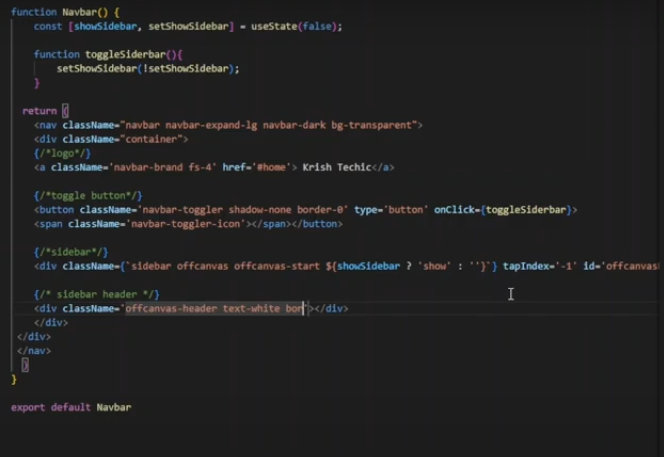
\includegraphics[width=0.5\textwidth]{..//uploads/1740076455021.PNG}
\caption{Fig 3 code}
\end{figure}





  \section{Results / Discussion}
  To provide an efficient writing experience, the third stage introduces a form-based user interface (UI) using Quill.js in a collaborative research environment. This interface allows authors to create structured sections, write content in a flexible text editor, and request AI-driven enhancements. Authors can select specific text for AI-based refinement or submit the entire document at once for a full academic transformation. The UI also enables real-time collaboration, allowing multiple researchers to work on the document simultaneously while maintaining content integrity and academic structure. The AI model strictly focuses on academic text refinement, while document formatting is handled separately by the IEEE-compliant LaTeX template.
In the fourth stage, the AI-refined content is applied to a LaTeX-based IEEE template to ensure proper document formatting, layout consistency, and citation structuring. The LaTeX template enforces IEEE formatting standards, using Times New Roman (10pt) in a double-column format for body text. Section titles are formatted in bold 12pt font, while subsection titles use bold 11pt font, ensuring clear document hierarchy. Figures and tables are automatically structured, labeled, and numbered according to IEEE standards, ensuring accuracy. Mathematical equations are formatted within LaTeX mathematical environments, maintaining IEEE compliance. References are structured using IEEE citation styles, ensuring proper in-text citation and bibliography formatting without requiring manual adjustments.
Finally, the system undergoes a validation process to ensure the document meets IEEE compliance standards before final export. The AI performs proofreading and coherence analysis, verifying academic tone, grammatical accuracy, and logical flow. The system also validates section structuring, citation accuracy, and reference formatting to prevent inconsistencies. Once validated, the document is automatically exported as a LaTeX-generated IEEE-compliant PDF, providing a submission-ready research paper.
By integrating AI-driven academic writing enhancement with automated LaTeX-based formatting, this system reduces the manual effort required for research writing, ensures IEEE compliance, and enhances writing clarity and consistency. The proposed method bridges the gap between AI-assisted writing and structured academic publishing, making research documentation faster, more efficient, and standardized for professional submissions.





  

  

  




\begin{thebibliography}{1}

  
    \bibitem{ref-1740062965592}
    
  

\end{thebibliography}

\end{document}
